% !TeX root = ../../pythonTutorial.tex
\section{Formatierung von Strings}
\label{formatInOut}

Es w�re sicherlich hilfreich, wenn wir die String-Ausgaben nach belieben formatieren k�nnten. Bisher haben wir den Seperator von \emph{print()} kennengelernt - dieser ist von seiner Funktionsweise jedoch stark beschr�nkt. Python bietet uns hierf�r die \emph{format()}-Methode an, vorher betrachten wir aber die Modulo-Arithmetik und machen uns mit den Formatierungszeichen vertraut.
 
Mittels Modulo-Arithmetik \randnotiz{Modulo-
Arithmetik} leiten wir ein Formatierungszeichen ein. Dieses gilt als Platzhalter f�r einen Wert.

\begin{lstlisting}[language=Python, label=formatInOut:lst:modulo]
# Modulo-Arithmetik

print("K�rper: %s , Fl�che: %f m" %
	('Dreieck', 42.6))
	
# Ausgabe:
# K�rper: Dreieck , Fl�che: 42.6
\end{lstlisting}

Bei "'K�rper"' setzen wir den ersten Platzhalter mit "'\%s"'. Die Reihenfolge der Platzhalter setzt fest, welcher Wert anschlie�end eingebunden wird. Der erste Platzhalter tr�gt also den ersten Wert, der nach dem Ausgabetext folgt, der zweite den zweiten und so weiter.

\warning{Die einzusetzenden Werte werden nach dem String mittels Modulo als Tupel festgelegt!}

Das Formatierungszeichen nach dem Modulo bestimmt den Datentyp des Wertes.
Bei "'s"' handelt es sich um einen String, bei "'f"' um ein \emph{float}.
In folgender Tabelle sind die m�glichen Formatierungszeichen aufgelistet.

\begin{figure}
	\caption{Formatierungszeichen und ihre Bedeutung \cite{pythonFormat}}
	\centering
	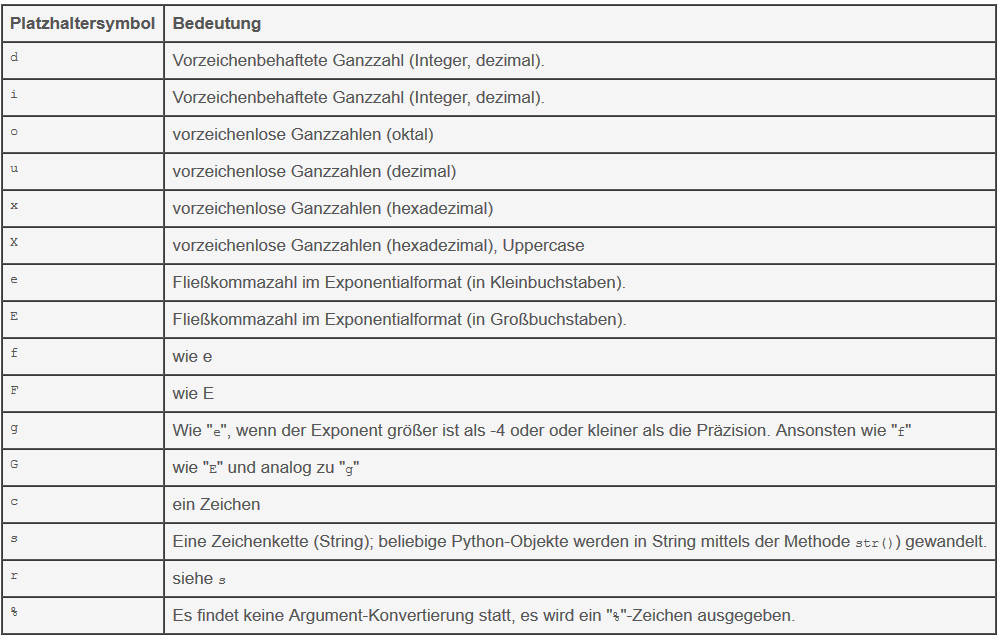
\includegraphics[width=\textwidth]{chapters/inputOutput/FormatierungSymbole.png}
\end{figure}

Was ist jedoch, falls die Ausgabe eine bestimmte L�nge haben soll?
Mit Hilfe der Syntax der Modulo-Arithmetik k�nnen wir dieses Problem l�sen.

 \begin{lstlisting}[language=Python, label=formatInOut:lst:syntax]
 # Modulo-Arithmetik Syntax
 
%[Flag][Minimum der Gesamtl�nge].[Pr�zision][Typ]
 \end{lstlisting}
 
 Das Minium der Gesamtl�nge bringt gro�e Vorteile mit sich, wenn wir z.B. einen linksb�ndigen Text ausgeben wollen. Alle Ausgaben, die k�rzer als das vorgegebene Minimum sind, werden mit Leerzeichen aufgef�llt.
 
 \warning{Es handelt sich hierbei um das Minimum der Gesamtl�nge. Alle Ausgaben die gr��er sind, werden nicht beschr�nkt und in voller L�nge ausgegeben!}
 
 Mittels Punkt k�nnen wir folgend die Pr�zision einstellen, was bei einem \emph{Float}-Datentyp die Nachkommastellen bestimmt. Alle Zahlen werden zu der angegebenen Nachkommastelle aufgerundet!
 
  \begin{lstlisting}[language=Python, label=formatInOut:lst:precision]
 # Modulo-Arithmetik Pr�zision
 
print("Eine Zahl %f" % (1.234))
print("Eine gerundete Zahl %.2f)

# Ausgabe:
# Eine Zahl 1.234
# Eine gerundete Zahl 1.23
 \end{lstlisting}
 

\begin{tabular}{|c | p{8cm}|}
	\hline
	Formatierungsanweisung & Bedeutung \\
	\hline
	< & Text wird linksb�ndig ausgelegt \\
	> & Text wird rechtsb�ndig ausgelegt \\
	\hline
\end{tabular}

